\section{Projections}\label{proj}
With the core functionality of \texttt{Blossom} described in the previous section, \textit{\nameref{proto}} [\S\ref{proto}], we may move on to the theoretical analysis of the protocol. In this section, we will describe models related to different performance characteristics of \texttt{Blossom}, as to project their theoretical performance before real-world testing. It is important that prior to the protocol passing any real-world examination, there are no fundamental issues we discover during our theoretical examination.

The performance categories we will be modeling in this section, include the \textit{\nameref{proj:tps}} [\S\ref{proj:tps}], \textit{\nameref{proj:ft}} [\S\ref{proj:ft}], \textit{\nameref{proj:fb}} [\S\ref{proj:fb}], and \textit{\nameref{proj:dyn_ut}} [\S\ref{proj:dyn_ut}]. These metrics represent the fundamental features of a successful blockchain protocol, with the ideal outcome displaying the protocol's ability to provide consistently high performance while maintaining a strong tolerance to byzantine behavior. While there do not exist clear standards to classify the success or failure of the protocol relative to any of these single metrics, we can estimate the performance of our system against precedent networks.

\subsection{Protocol Throughput and Finality}\label{proj:tps}
As a uniquely scalable consensus protocol, we expect the performance of \texttt{Blossom} will be limited by infrastructure conditions rather than a fundamental behavior within the protocol. This results in a theoretical maximum network throughput which is determined by non-protocol features, such as IT infrastructure and node hardware. When developing a model to estimate the performance of our protocol we implemented the following variables: compute threads (\textit{t}), bandwidth [MB/s] (\textit{b}), the latency per round in an open channel [ms] (\textit{l}), transactions per block (\(\beta\)), transaction size [bytes] (\(\tau\)), signature verifications per second per thread (\(\nu\)) and average block efficiency (\textit{E}). We recognize there exist possible variances between these variables and their real-world outcome; however, the purpose of this model is to approximate general performance outcomes over scales, rather than predict exact performance. With the above variables block time (\(B_t\)) and throughput (\textit{T}) are as follows, given nodes (\textit{n}):
\[
B_t =
(5.5n \times 10^{-7})
+
\frac{\beta n E \tau}{b}
+
\tfrac{\beta n E+n+\big(n\log_q(n) \big)}{\nu t}
+
\big (l \times \lceil \log_q(\tfrac{n}{2}) \rceil \big)
\]
\[
T = \frac{\beta n E}{B_t}
\]

Due to the protocol's cooperative nature, the values inserted for each variable are expected to represent the characteristics of the bottom 33\% of nodes (i.e. least performant…) members of the network, as it is these members who bottleneck the throughput of the entire platform. This mitigates any performance overestimation returned by the model associated with the selection of median or average performance. A reasonable expectation of the least viable system would be a node with the hardware and infrastructure attributes equivalent to an Intel Core i5-10400 CPU and an internet bandwidth (upload \& download) of 10 MB/s.

When accounting for the above processor and bandwidth characteristics, with the additional expected base values for the remaining variables, we are provided the following inputs for our model \(
\{
t = 8, \
b = 10, \ 
l = 200, \
\beta = 1000, \
\tau = 200, \
\nu = 20000 \
E = 1.00
\}
\).

\begin{figure}[h!]
    \centering
    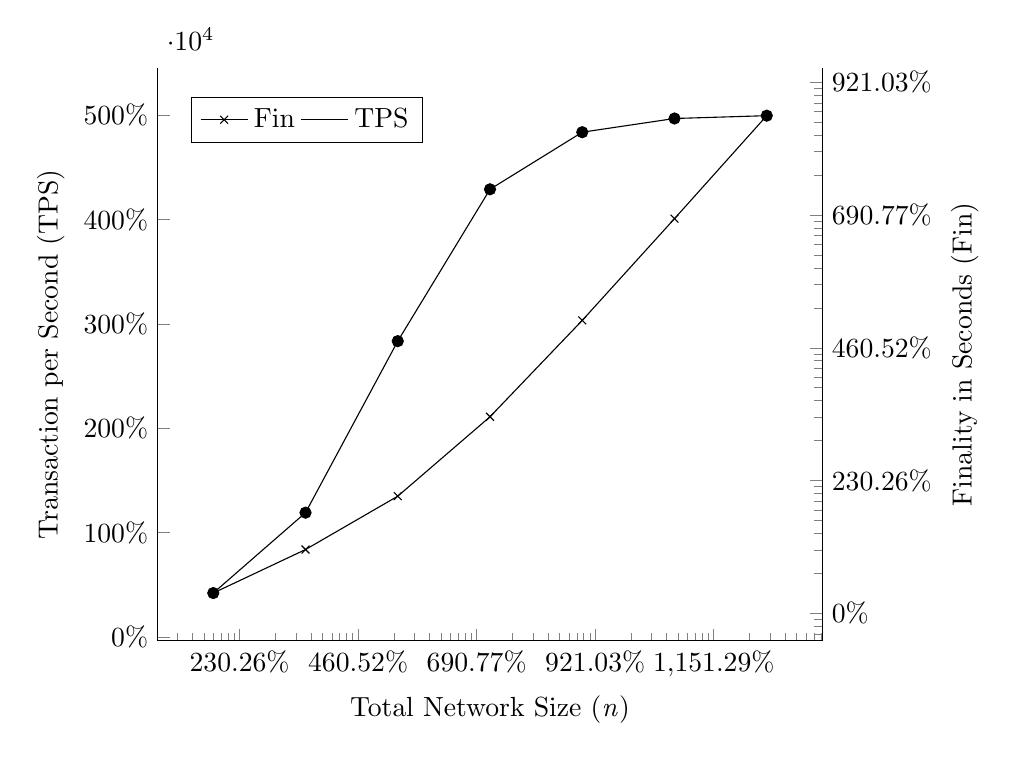
\begin{tikzpicture}
      \pgfplotsset{
          scale only axis,
      }
    
      \begin{axis}[
        xmode=log,
        axis y line*=left,
        axis x line*=bottom,
        xlabel = Total Network Size (\textit{n}),
        ylabel= Transaction per Second (TPS),   
        scaled y ticks=true
      ]
        \addplot[mark=*]
          coordinates{
            (6,4225.35)	
            (36,11920.49)	
            (216,28346.26)	
            (1296, 42885.46)	
            (7776,48351.61)	
            (46656,49664.07)	
            (279936,49934.27)
            % more points
          }; \label{plot_1}
    
        \end{axis}
    
        \begin{axis}[
          xmode=log,
          ymode=log,
          axis y line*=right,
          axis x line*=bottom,
          axis x line=none,
          ylabel=Finality in Seconds (Fin),
          legend style={at={(0.05,0.95)}, anchor=north west, legend cell align=left},
        ]
    
        \addplot[mark=x]
          coordinates{
            (6,1.42)	
            (36,3.02)	
            (216,7.62)	
            (1296, 30.22)	
            (7776,160.82)	
            (46656,939.43)	
            (279936,5606.09)			
            % more points
          }; \label{plot_2}
        \addlegendimage{/pgfplots/refstyle=plot_1}\addlegendentry{Fin}
        \addlegendimage{/pgfplots/refstyle=plot_2}\addlegendentry{TPS}
        \end{axis}
    \end{tikzpicture}
    \caption{The network throughput and finality as the number of network members increases, assuming the network is under maximum possible load.}
    \label{fig:proj_small}
\end{figure}

In analyzing \textit{Figure} \ref{fig:proj_small} it becomes clear that as the number of nodes increases, which occurs exponentially at intervals of \(q^x\), the throughput of the network reaches a maximum limit \([\approx 50,000]\), while the finality for all applicable transactions increases at a rate highly correlated to a linear coefficient \([R^2 = 0.9782]\).

We believe these results to be accurate due to the known bottlenecks of the protocol, with those bottlenecks being network bandwidth and compute potential. Bandwidth is considered a reasonable bottleneck as every transaction has a minimum viable size, and as the number of transactions increases, there is a linear increase in latency. Compute potential is another reasonable bottleneck as every transaction stores a cryptographic signature, with said signature having a high compute cost. When a transaction is added to the ledger the signature must first be validated, and as the number of signatures increases there is a linear increase in latency. Beyond bandwidth and compute potential other minor bottlenecks exist; however, these two factors account for a majority (\(>99\% \)) of all protocol latency. While protocol-specific improvements will be discussed in later sections [see \S\ref{conclusion}], IT improvements provide the greatest potential performance increases. Accounting for the previous model variables, if the  estimated network bandwidth was improved by a factor of two (2) to support \(\{ b = 20\}\), we would see a throughput improvement of \([\approx100\%]\) while time to finality would be reduced by \([\approx50\%]\) when compared to the values used in \textit{Figure} \ref{fig:proj_small}. When accounting for an average system with the variables of \(\{
t = 16, \
b = 100 
\}\)  we would see a throughput improvement of \([\approx550\%]\) while time to finality would be reduced by \([\approx85\%]\) when compared to the values used in \textit{Figure} \ref{fig:proj_small}.

When placing our protocol in the context of the decentralized ecosystem, we can observe the characteristics of precedent networks, as to reference the distribution of node hardware represented in active systems. When observing the Ethereum network, there are 4797 active nodes, with an estimated \(63.8\%\) of said nodes hosted in the cloud — a majority of which are hosted on AWS \cite{ether-nodes-hz}. Ignoring the negative consequences of this decentralization, if \texttt{Blossom} nodes were hosted in the cloud to an equivalent degree as on Ethereum, we would be able to drastically increase projected performance, due to the high bandwidth of cloud infrastructure and rapid scalability of cloud compute. Referencing the metrics for standard cloud services, we see \(
\{
t \ge 32, \
b \ge 10000 
\}
\). If we were to re-compute our model with the new metrics \(
\{
t = 32, \
b = 10000 
\}\) we would observe a new distribution, as seen in \textit{Figure} \ref{fig:proj_large}. 

\begin{figure}[h!]
    \centering
    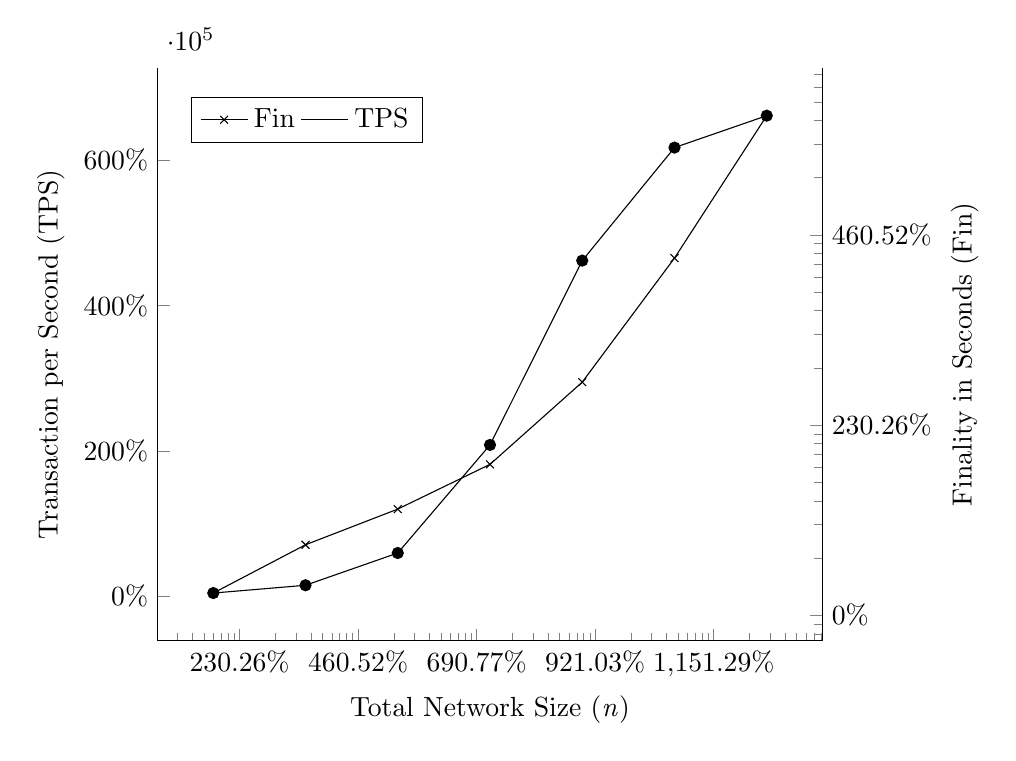
\begin{tikzpicture}
      \pgfplotsset{
          scale only axis,
      }
    
      \begin{axis}[
        xmode=log,
        axis y line*=left,
        axis x line*=bottom,
        xlabel = Total Network Size (\textit{n}),
        ylabel= Transaction per Second (TPS),   
        scaled y ticks=true
      ]
        \addplot[mark=*]
          coordinates{
            (6,4584.13)	
            (36,15298.09)	
            (216,59673.05)	
            (1296, 208362.67)	
            (7776,461963.52)	
            (46656,617451.49)	
            (279936,661354.75)
            % more points
          }; \label{plot_1}
    						
        \end{axis}
    
        \begin{axis}[
          xmode=log,
          ymode=log,
          axis y line*=right,
          axis x line*=bottom,
          axis x line=none,
          ylabel=Finality in Seconds (Fin),
          legend style={at={(0.05,0.95)}, anchor=north west, legend cell align=left},
        ]
    
        \addplot[mark=x]
          coordinates{
            (6,1.31)	
            (36,2.35)	
            (216,3.62)	
            (1296, 6.22)	
            (7776,16.83)	
            (46656,75.56)	
            (279936,423.28)			
            % more points
          }; \label{plot_2}
        \addlegendimage{/pgfplots/refstyle=plot_1}\addlegendentry{Fin}
        \addlegendimage{/pgfplots/refstyle=plot_2}\addlegendentry{TPS}
        \end{axis}
    \end{tikzpicture}
    \caption{The network throughput and finality as the number of network members increases, assuming the network is under maximum possible load.}
    \label{fig:proj_large}
\end{figure}

The new projection displayed in Figure 2 is much more impressive than that displayed in Figure 1, as the bandwidth allowance was increased by 100x. As a consequence, when compared to Figure 1 we have seen a throughput improvement of \([\approx1340\%]\) while time to finality is reduced by \([\approx93\%]\). When isolating this performance increase to the equivalent network values displayed by Ethereum, of 4797 active nodes, the model projects a throughput performance of 462,743 TPS at a finality time of 16.8 seconds.
From the observation of the necessary performance required of functioning platforms, the performance displayed in both \textit{Figure} \ref{fig:proj_small} and \textit{Figure} \ref{fig:proj_large} are comparable to sustainable and efficient infrastructure, especially given \texttt{Blossom} is able to achieve this performance with non-specialized hardware.

\subsection{Fault Tolerance}\label{proj:ft}
It is important we clarify that the fault tolerance noted for each quorum and the fault tolerance of each epoch (e.g. each state) are not required to be equivalent, and whether the two thresholds are represented by a similar fault ratio or not, there is no programmatic need for parity. That being said, as to avoid confusion we will refer to the fault tolerance of each quorum as the ‘quorum fault tolerance,’ and the fault tolerance of each epoch as the ‘epoch fault tolerance.’ Previous BFT-based protocols have laid the groundwork in designed a protocol that is capable of reaching consensus amongst a distributed network using P2P network dynamics; however, as each quorum is but a partition of the greater network, to guarantee a global consensus we must undergo more rigorous proofs. In this section, we will be focusing on the methodology for achieving said proofs, as well as quantifying the methods for maintaining a consensus.

The \textit{epoch fault tolerance} we have chosen to implement for our protocol requires a supermajority consensus of greater than \(\frac{2n}{3}\) nodes. Our reason for selecting this value is due to its leniency, allowing for the presence of a reasonable number of byzantine nodes before consensus no longer occurs (\(\frac{n}{3}\)), and that this fraction has the smallest integer numerator and denominator while greater than a \(50\%\) equality. We have chosen to avoid a regular majority consensus (\(> 50\%\)), as the threshold may be too exact for our style of distributed protocol. If a more cautious approach were taken, we would recommend increasing the \textit{epoch fault tolerance} to require a supermajority consensus of greater than \(\frac{3n}{4}\) or  nodes. Once a limit has been selected we can verify if a given state has been reached rather easily, by querying the historic epoch hash of every node at a specified epoch nonce. We used the term ‘historic’ when describing this querying method, as this approach would be highly inefficient if implemented for nodes participating in consensus. This inefficiency would decrease our actual finality time, thus negatively affecting our TPS measurement. Following the completion of a given Epoch, we verify if a supermajority consensus did or did not occur by surveying the purported ‘last epoch’  stored within every novel block, checking if the total number of blocks with a shared epoch is greater or less than the \textit{epoch fault tolerance} required by the network. The procedure of verifying the ‘last epoch’ stored within each block header is already completed during both the \textit{block propagation} and transaction validation phase of \texttt{Blossom}; however, to verify fault tolerance we added the additional behavior of logging the number of blocks with an identical epoch hash. If a node determines that a consensus has not been reached, then it is their prerogative to ignore the outcome of their present epoch, and gossip across the network that they believe consensus has stalled. If this failure to convene is false, and the greater network did achieve consensus then the node will be seen as faulty by their peers; however, in the case, it is true that consensus failed to occur, nodes will begin attempting to \textit{restate} the network.

The \textit{restate} protocol has nodes randomly subsample the entire network, creating novel quorums of size \textit{q}. The goal of each quorum is to quickly determine the most recent epoch nonce where a supermajority of nodes has an identical state. The quorum members will then adopt that epoch as their new ‘most recent’ epoch. As we cannot remove epochs that have already been verified with a supermajority consensus, it is expected that nodes will only be required to move back one (1) nonce from their present position; however, given nodes may have incorrectly formed several epochs we provide nodes the ability to move back further than one (1) epoch. The specifics of the \textit{restate} protocol deserve their own paper; however, we expect enough to be gleaned from this short summary to recognize the role and significance of the procedure.

For a \textit{restate} to occur there must be some number of byzantine nodes present in the network. Due to factors we have discussed previously, and will discuss in a coming section (see \textit{\nameref{proj:fb}} [\S\ref{proj:fb}]), it is necessary that byzantine nodes are pruned from the greater network in a means which is both uncontroversial and able to occur concurrently across a supermajority of distributed nodes. It is important that the implementation mitigates Type I errors, and the dismissal of non-byzantine nodes, and as such it is important nodes are acted upon in a verifiable fashion. The three variant solutions we propose are each reasonable approaches to resolve this issue; however, each maintains a unique distribution of tradeoffs that may or may not dissuade said solutions' implementation. The three solutions we propose are: 

\begin{description}
\item[Pruning by an arbiter,] refers to the use of a specialized node that observes network behavior and develops proof against observed byzantine nodes. This proof should be easily verified by all parties, with the arbiter themselves held in high regard. This system is similar to the use of a fisherman, described in the Polkadot whitepaper \cite{polkadot-pl}. However, to elaborate on the specific behaviors of an arbiter within \texttt{Blossom}, their behavior would be the following. Similar to light nodes or replica nodes, each arbiter would maintain a local replica of the network state which would be updated each epoch. This state is expected to be valid, with the appropriate amount of signatures maintained with the associated epoch. To develop a proof against an operating node, an arbiter would be tasked with auditing the historical record of every blockchain node, as to check for faults against their local record. The methods by which an arbiter checks the record are up to their digression; however, it is the arbiter’s responsibility to return verifiable proof quantifying a pattern of byzantine behavior. As all nodes are required to present cryptographic signatures with the presentation of any novel data (e.g. blocks and epochs), if a node did operate in a provably byzantine manner, the record should maintain proof of the node ratifying the faulty state with their signature.
\item[Pruning by incorrect consensus,] refers to the concurrent decision by nodes to remove their peers who did not reach an identical supermajority consensus as the greater network. This is expected to occur immediately following the discovery of such a lapse (i.e. the epoch following the fault’s occurrence), with no tolerance for accidental deviations from the greater network. This approach is highly punitive to nodes who presented Byzantine behavior for non-malicious reasons and offers no opportunity for Byzantine nodes to independently correct their state. This lack of tolerance is especially important given the presence of finical or social disincentives which are adopted following a node's removal. We would only recommend this procedure's inclusion in the pruning process if it is discovered that the risk of allowing byzantine nodes to linger on the network is immense.
\item[Pruning by observed byzantine behavior,] is similar to the previous solution (pruning by incorrect consensus); however, rather than immediately removing nodes found to be purporting an incorrect state, some pattern is required to be observed over a series of sequential epoch’s for a node to be pruned. This approach would allow non-byzantine nodes the opportunity to independently correct their state without punishment, while byzantine nodes are removed due to their observed faulty behavior. The barriers to adopting this approach are due to the computation required to develop a ‘proof of fault’ in the required manner. It may be unfeasible for nodes to observe and log their peer's behavior concurrent with participating in consensus. If the threshold of proof would require a supermajority of nodes to personally participate in a quorum with some byzantine node, said byzantine node would remain an active member of the network for \(\frac{n}{(q-1) \times \log_q(n)}\) epochs in the best case scenario. There exists little value in the firsthand account of byzantine behavior due to the use of cryptographic signatures; however, the question then arises: ‘If byzantine nodes are not removed immediately, what threshold merits their expulsion?’
\end{description}

When looking to adopt these three approaches we recognize it will be important to test the viability of each method in a reasonable manner; however, given the issues which may arise as a result of strategic byzantine nodes (malicious nodes) as well as regular byzantine nodes, we expect our solution will require both the use of an arbiter and distributed pruning process. We may also discover additional methods for resolving the pruning of byzantine nodes, and we intend on disclosing such novel methods in future documentation given the need may arise.

\subsection{Failure Bleed}\label{proj:fb}
Earlier in this paper we introduced the concept of a \textit{failure bleed}, the ability for byzantine nodes to induce faulty behavior in non-byzantine nodes by blocking consensus, or not sharing correct information. To reduce the occurrence of \textit{failure bleed}, we introduced a second recursion of the consensus tree, allowing nodes to reconvene with their past quorums to verify data concurrency before finalizing the epoch state. At the cost of additional latency during consensus, this solution drastically reduces the likelihood of a \textit{failure bleed} to occur. To quantify this difference before and after the introduction of this solution, we must acknowledge the reasons a \textit{failure bleed} may occur, so as to guarantee its mitigation.

In the original approach, with a single recursion of the consensus tree, it is required that every quorum a node participates in reaches consensus. If a consensus is not reached, each non-byzantine quorum member will experience some data loss. This means that given the number of faulty nodes in a quorum is greater than the fault tolerance of each quorum \((f > \frac{1}{3})\), then all remaining nodes in that quorum will become faulty as well. With the more tolerant approach, due to the additional recursion of the consensus tree, as long as a node participated in at least one (1) quorum which successfully reached consensus, they will most likely be able to resolve any data loss they maintain. To measure the probability that a \textit{failure bleed} (\textit{F}) were to occur in this scenario, we will be testing for the maximum number of non-byzantine nodes who become byzantine, assuming \textit{n} represents all nodes on the network, \textit{f} represents the total number of byzantine nodes on the network, and \textit{a} represents the minimum number of faults required for all quorums to be considered faulty. The formula for determining the likelihood that {\(\frac{f}{a}\) \textit{failure bleed’s} occur is as follows:
\[
a = \big (
\lfloor
\frac{q}{3}
\rfloor +1 \big )
\times
\big ( \log_q(n)-1 \big)
\]
\[
F =\prod ^{
\lfloor
\frac{f}{a}\rfloor
}
_{i=0} \bigg(
\prod _{j=0}^{a} \tfrac{(f-ai)-j}{(n-ai)-j} 
\bigg)
\]

Implementing these functions over the network of sizes \(n=6^{[2:6]}\), we can observe the maximum likelihood that non-byzantine nodes become byzantine as a consequence of \textit{failure bleed}. We then plotted these results in \textit{Figure} \ref{fig:failure_f3} and \textit{Figure} \ref{fig:failure_f6} with each graph representing the probability that one (1) through five (5) new faults occur due to \textit{failure bleed}. Our reason for distributing these measurements was to quantity the probabilistic effect of a network with more or less byzantine nodes present. To quantify this variance \textit{Figure} \ref{fig:failure_f3} expects the network to maintain \(f=\frac{n}{3}\) byzantine nodes, while \textit{Figure} \ref{fig:failure_f6} has the network maintain \(f=\frac{n}{6}\) byzantine nodes. In reducing the number of byzantine number of nodes across the network we expect the likelihood of \textit{failure bleed} to reduce, at a non-linear rate.


\begin{figure}[h!]
    \centering
    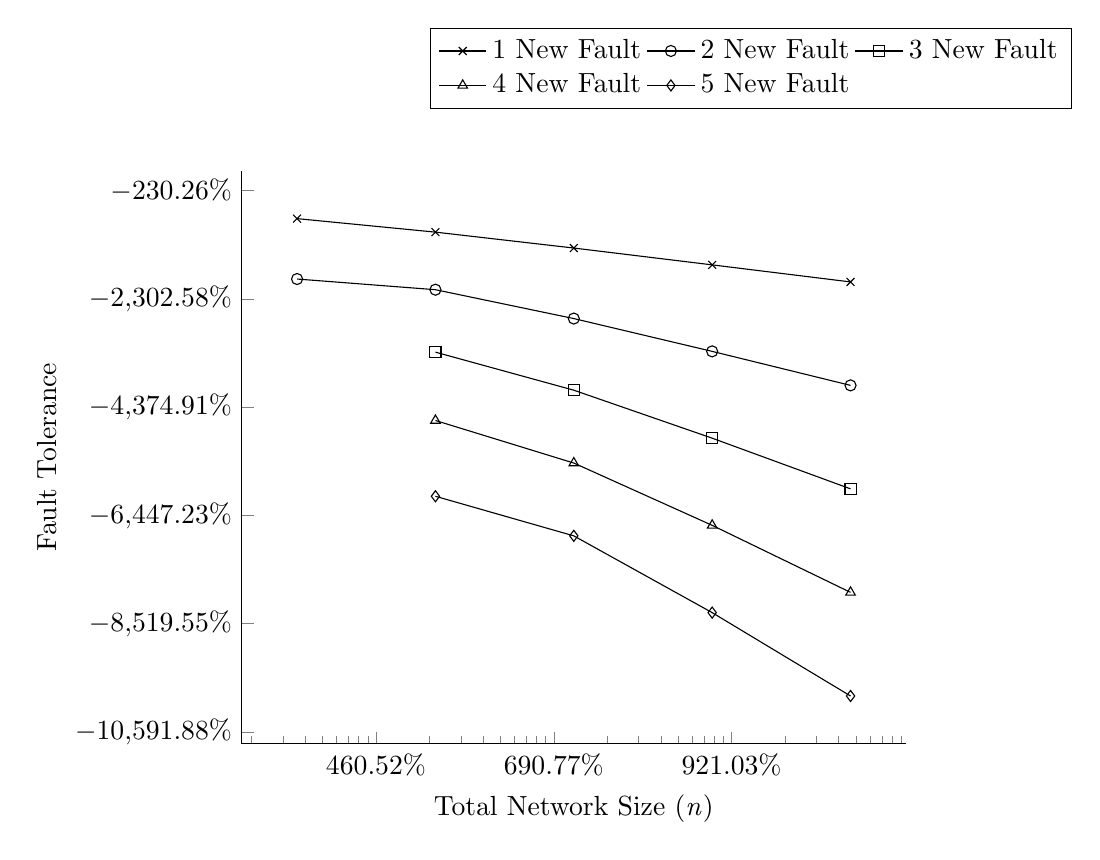
\begin{tikzpicture}
      \pgfplotsset{
          scale only axis,
          every axis legend/.append style={ at={(1.25,1.25)}, 
          legend columns = 3}
      }
    
      \begin{axis}[
        xmode=log,
        ymode=log,
        axis y line*=left,
        axis x line*=bottom,
        xlabel = Total Network Size (\textit{n}),
        ylabel= Fault Tolerance,   
        scaled y ticks=true
      ]
        \addplot[mark=x,color=black] coordinates{
            (36,0.000474)	
            (216,0.0000357)	
            (1296, 0.0000017)	
            (7776,0.0000000678)	
            (46656,0.00000000259)	
            % more points
          }; \label{plot_1_y1}
    
        \addplot[mark=o,color=black] coordinates{
            (36,0.00000000451)	
            (216,0.000000000584)	
            (1296,0.00000000000233)	
            (7776,0.00000000000000436)	
            (46656,0.00000000000000000649)	
            % more points
          }; \label{plot_1_y2}
          
        \addplot[mark=square,color=black] coordinates{
            (216,0.00000000000000376)	
            (1296,0.00000000000000000258)	
            (7776,0.000000000000000000000265)	
            (46656,0.0000000000000000000000000162)	
            % more points
          }; \label{plot_1_y3}
        
        \addplot[mark=triangle,color=black] coordinates{
            (216,0.00000000000000000000781)	
            (1296,0.00000000000000000000000227)	
            (7776,0.000000000000000000000000000015)	
            (46656,0.00000000000000000000000000000000004)	
            % more points
          }; \label{plot_1_y4}
        
        \addplot[mark=diamond,color=black] coordinates{
            (216,0.00000000000000000000000000391)	
            (1296,0.000000000000000000000000000002)	
            (7776,0.00000000000000000000000000000000000083)	
            (46656,0.0000000000000000000000000000000000000000000972)	
            % more points
          }; \label{plot_1_y5}
          \addlegendimage{/pgfplots/refstyle=plot_1_y1}\addlegendentry{1 New Fault}
        \addlegendimage{/pgfplots/refstyle=plot_1_y2}\addlegendentry{2 New Fault}
        \addlegendimage{/pgfplots/refstyle=plot_1_y3}\addlegendentry{3 New Fault}
        \addlegendimage{/pgfplots/refstyle=plot_1_y4}\addlegendentry{4 New Fault}

        \addlegendimage{/pgfplots/refstyle=plot_1_y4}\addlegendentry{5 New Fault}
        \end{axis}
    \end{tikzpicture}
    \caption{The likelihood that a new node would become faulty due to \textit{failure bleed} given \(f = \frac{n}{3}\) faulty nodes.}
    \label{fig:failure_f3}
\end{figure}
\begin{figure}[h!]
    \centering
    \begin{tikzpicture}
      \pgfplotsset{
          scale only axis,
          every axis legend/.append style={ at={(1.25,1.25)}, 
          legend columns = 3}
      }
    
      \begin{axis}[
        xmode=log,
        ymode=log,
        axis y line*=left,
        axis x line*=bottom,
        xlabel = Total Network Size (\textit{n}),
        ylabel= Fault Tolerance,   
        scaled y ticks=true
      ]

        \addplot[mark=x,color=black] coordinates{
            (36,0.000000513)	
            (216,0.0000000395)	
            (1296, 0.000000000345)	
            (7776,0.00000000000199)	
            (46656,0.00000000000000969)	
            % more points
          }; \label{plot_1_y1}
    
        \addplot[mark=o,color=black] coordinates{
            (216,0.000000000000000162)	
            (1296,0.000000000000000000073)	
            (7776,0.00000000000000000000000344)	
            (46656,0.0000000000000000000000000000908)	
            % more points
          }; \label{plot_1_y2}
          
        \addplot[mark=square,color=black] coordinates{
            (216,0.0000000000000000000000000231)	
            (1296,0.00000000000000000000000000000845)	
            (7776,0.0000000000000000000000000000000000052)	
            (46656,0.000000000000000000000000000000000000000000823)	
            % more points
          }; \label{plot_1_y3}
        
        \addplot[mark=triangle,color=black] coordinates{
            (216,0.0000000000000000000000000000000000000063)	
            (1296,0.000000000000000000000000000000000000000527)	
            (7776,0.00000000000000000000000000000000000000000000000682)	
            (46656,0.00000000000000000000000000000000000000000000000000000000722)	
            % more points
          }; \label{plot_1_y4}
        
        \addplot[mark=diamond,color=black] coordinates{
            (1296,0.000000000000000000000000000000000000000000000000017)	
            (7776,0.00000000000000000000000000000000000000000000000000000000000776)	
            (46656,0.0000000000000000000000000000000000000000000000000000000000000000000000613)	
            % more points
          }; \label{plot_1_y5}
          \addlegendimage{/pgfplots/refstyle=plot_1_y1}\addlegendentry{1 New Fault}
        \addlegendimage{/pgfplots/refstyle=plot_1_y2}\addlegendentry{2 New Fault}
        \addlegendimage{/pgfplots/refstyle=plot_1_y3}\addlegendentry{3 New Fault}
        \addlegendimage{/pgfplots/refstyle=plot_1_y4}\addlegendentry{4 New Fault}

        \addlegendimage{/pgfplots/refstyle=plot_1_y4}\addlegendentry{5 New Fault}
        \end{axis}
    \end{tikzpicture}
    \caption{The likelihood that a new node would become faulty due to \textit{failure bleed} given \(f = \frac{n}{6}\) faulty nodes.}
    \label{fig:failure_f6}
\end{figure}

\subsection{Dynamic Utilization}\label{proj:dyn_ut}
The performance measurements we reference in \textit{\nameref{proj:tps}} [\S\ref{proj:tps}], as well as other moments later in this document, were projected or collected when the network was operating within the range of ‘maximum utilization.’ \textit{Maximum utilization} refers to the characteristic of a given epoch where at least \(90\%\) of possible transactions which may be distributed are distributed (\(\ge 90\%\)). This classification is important due to our use of a block cap, limiting the total number of transactions each node may distribute in a given epoch. For sake of example, given a network of 1,000 nodes (\(n=1000\)) with a block limit equivalent to 1,000 transactions (\(\equiv 1000\)), then the \textit{maximum utilization} range for each epoch would be 900,000 to 1,000,000 transactions.

Due to the scalability of \texttt{Blossom}, and previously discussed dynamics of the block limit, we expect the real-world utilization of \texttt{Blossom} to run well below \textit{maximum utilization}. In the realistic scenario where network utilization is dynamic, we are interested in understanding the effect such fluctuations may have on overall network performance if any effect is had at all.

For this analysis, we will make use of the model we developed in the section \textit{\nameref{proj:tps}} [\S\ref{proj:tps}], as to represent the effect on performance from variations in network utilization. To display changes over scale, we will measure network utilization ($U$), which is equivalent to \textit{average block efficiency} (\(U \equiv E\)), and the size of the network (\textit{n}). Network utilization will be measured in intervals of \(10\%\), while changes to the number of network members will be tested with 100, 1,000, and 10,000 nodes.



\begin{figure}[h!]
    \centering
    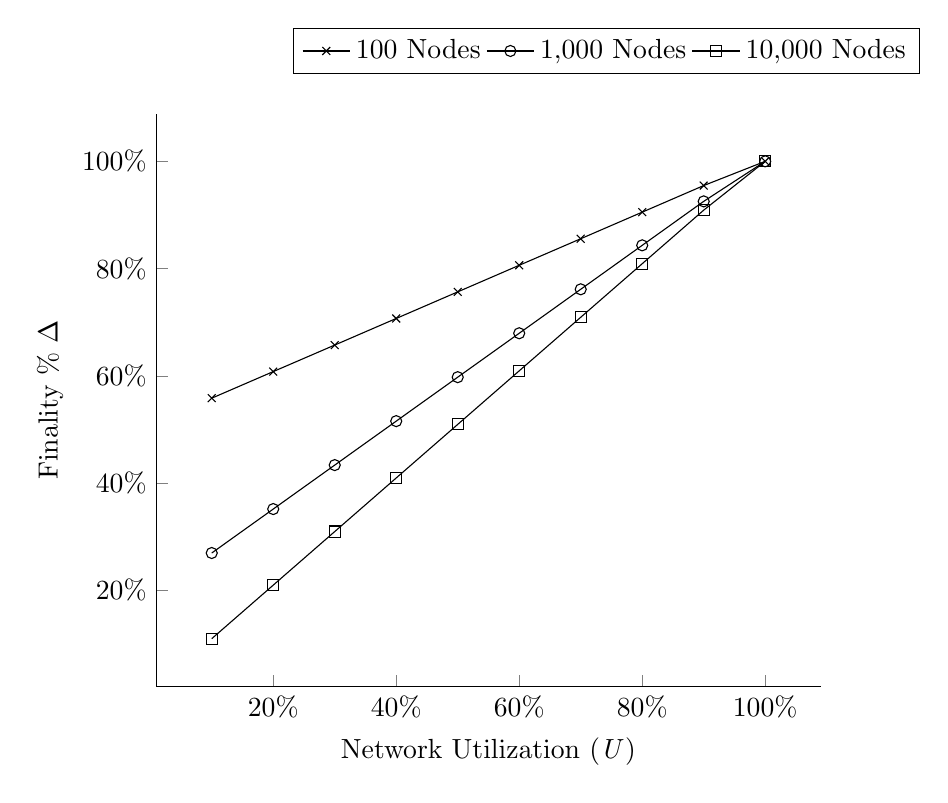
\begin{tikzpicture}
      \pgfplotsset{
          scale only axis,
          xticklabel={\pgfmathparse{\tick*100}\pgfmathprintnumber{\pgfmathresult}\%},
          yticklabel={\pgfmathparse{\tick*100}\pgfmathprintnumber{\pgfmathresult}\%},
          every axis legend/.append style={ at={(1.15,1.15)}, 
          legend columns = 0}
          % legend style={at={(0.5,0.5)},
      }
    
      \begin{axis}[
        % xmode=log,
        % ymode=log,
        axis y line*=left,
        axis x line*=bottom,
        xlabel = Network Utilization (\textit{U}),
        ylabel= Finality \(\%\) \(\Delta\),   
        scaled y ticks=true
      ]

        \addplot[mark=x,color=black] coordinates{
            (1, 1)
            (.9,.9548)
            (.8,.9052)
            (.7,.8556)
            (.6,.8061)
            (.5,.7565)
            (.4,.7069)
            (.3,.6573)
            (.2,.6078)
            (.1,.5582)
            % more points
          }; \label{plot_1_y1}
    
        \addplot[mark=o,color=black] coordinates{
            (1, 1)
            (.9,.9253)
            (.8,.8433)
            (.7,.7613)
            (.6,.6793)
            (.5,.5974)
            (.4,.5154)
            (.3,.4334)
            (.2,.3514)
            (.1,.2694)
            % more points
          }; \label{plot_1_y2}
          
        \addplot[mark=square,color=black] coordinates{
            (1, 1)
            (.9,.9089)
            (.8,.809)
            (.7,.7091)
            (.6,.6092)
            (.5,.5093)
            (.4,.4094)
            (.3,.3094)
            (.2,.2095)
            (.1,.1096)
            % more points
          }; \label{plot_1_y3}

%           100 %	1	1	1
% 90 %	0.9548	0.9253	0.9089
% 80 %	0.9052	0.8433	0.809
% 70 %	0.8556	0.7613	0.7091
% 60 %	0.8061	0.6793	0.6092
% 50%	0.7565	0.5974	0.5093
% 40 %	0.7069	0.5154	0.4094
% 30 %	0.6573	0.4334	0.3094
% 20 %	0.6078	0.3514	0.2095
% 10 %	0.5582	0.2694	0.1096
        
        \addlegendimage{/pgfplots/refstyle=plot_1_y1}\addlegendentry{100 Nodes}
        \addlegendimage{/pgfplots/refstyle=plot_1_y2}\addlegendentry{1,000 Nodes}
        \addlegendimage{/pgfplots/refstyle=plot_1_y3}\addlegendentry{10,000 Nodes}

        \end{axis}
    \end{tikzpicture}
    \caption{The percentage decrease in finality time as \textit{network utilization} decreases.}
    \label{fig:fin_change}
\end{figure}


\begin{figure}[h!]
    \centering
    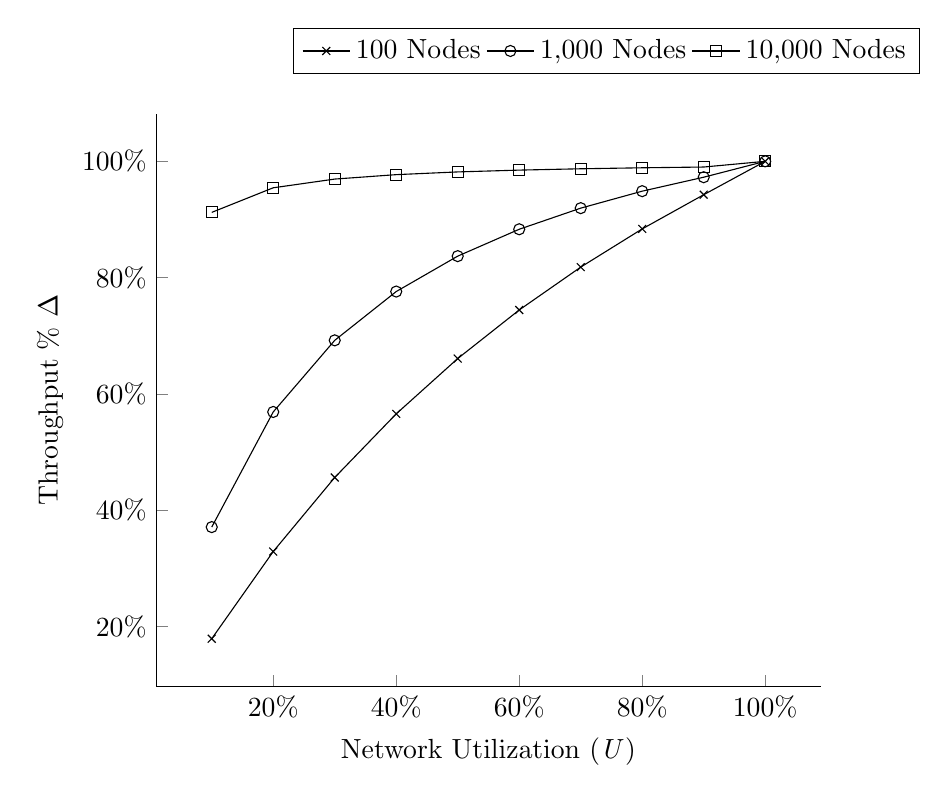
\begin{tikzpicture}
      \pgfplotsset{
          scale only axis,
          xticklabel={\pgfmathparse{\tick*100}\pgfmathprintnumber{\pgfmathresult}\%},
          yticklabel={\pgfmathparse{\tick*100}\pgfmathprintnumber{\pgfmathresult}\%},
          every axis legend/.append style={ at={(1.15,1.15)}, 
          legend columns = 0}
          % legend style={at={(0.5,0.5)},
      }
    
      \begin{axis}[
        % xmode=log,
        % ymode=log,
        axis y line*=left,
        axis x line*=bottom,
        xlabel = Network Utilization (\textit{U}),
        ylabel= Throughput \(\%\) \(\Delta\),   
        scaled y ticks=true
      ]

        \addplot[mark=x,color=black] coordinates{
            (1, 1)
            (.9,.9426)
            (.8,.8838)
            (.7,.8181)
            (.6,.7444)
            (.5,.6609)
            (.4,.5658)
            (.3,.4564)
            (.2,.3291)
            (.1,.1792)
            % more points
          }; \label{plot_1_y1}
    
        \addplot[mark=o,color=black] coordinates{
            (1, 1)
            (.9,.9727)
            (.8,.9487)
            (.7,.9195)
            (.6,.8832)
            (.5,.837)
            (.4,.7761)
            (.3,.6922)
            (.2,.5691)
            (.1,.3711)
            % more points
          }; \label{plot_1_y2}
          
        \addplot[mark=square,color=black] coordinates{
            (1, 1)
            (.9,.9902)
            (.8,.9889)
            (.7,.9872)
            (.6,.9849)
            (.5,.9818)
            (.4,.9771)
            (.3,.9695)
            (.2,.9545)
            (.1,.9122)
            % more points
          }; \label{plot_1_y3}

% 100 %	1	1	1
% 90 %	0.9426	0.9727	0.9902
% 80 %	0.8838	0.9487	0.9889
% 70 %	0.8181	0.9195	0.9872
% 60 %	0.7444	0.8832	0.9849
% 50%	0.6609	0.837	0.9818
% 40 %	0.5658	0.7761	0.9771
% 30 %	0.4564	0.6922	0.9695
% 20 %	0.3291	0.5691	0.9545
% 10 %	0.1792	0.3711	0.9122
        
        \addlegendimage{/pgfplots/refstyle=plot_1_y1}\addlegendentry{100 Nodes}
        \addlegendimage{/pgfplots/refstyle=plot_1_y2}\addlegendentry{1,000 Nodes}
        \addlegendimage{/pgfplots/refstyle=plot_1_y3}\addlegendentry{10,000 Nodes}

        \end{axis}
    \end{tikzpicture}
    \caption{The percentage decrease in finality time as \textit{network utilization} decreases.}
    \label{fig:tps_change}
\end{figure}

The outcome of this experiment presents that the rate of change for finality is linearly correlated with the rate of change in network utilization, as seen in \textit{Figure} \ref{fig:fin_change}, while the rate of change of throughput (TPS) is non-linearly correlated with the rate of change in network utilization, as seen in \textit{Figure} \ref{fig:tps_change}. In part due to the inverse relationship of throughput and finality, as well as other factors consequence of \texttt{Blossom} design, changes in network utilization have a relatively positive benefit for finality, as overall finality time is reduced, while the cost to throughput is diminished as the size of the network increases. This observation further supports the scalability claims of \texttt{Blossom}, as the network’s instability (i.e. the deviation of network throughput) is shown to decrease with the network’s size.

In cases where a network’s utilization is operating less than the protocol's maximum utilization threshold (\(< 90 \%\)), due to \texttt{Blossom} scalability efficiency decreases with network utilization, as seen in \textit{Figure} \ref{fig:tps_change} given TPS is directly correlated with per capital efficiency. With this being said, in circumstances where the \textit{network utilizing} \texttt{Blossom} is more averse to increases in finality than decreases in efficiency, there exists a moment of ‘ideal utilization.’ Implementing the formulas \(f(E)\) and \(g(E)\), where \(f(E)\) returns the finality of the network at given variables and \(g(E)\) returns the throughput of the network at given variables, we may find the ideal utilization of the network. When solving for network utilization, the formulas for \(f(E)\) and \(g(E)\) are as follows.

\[
f(E) = 
(5.5 \times 10^{-7})
+
\frac{\beta n E \tau}{b}
+
\frac{\beta E+n+(n\log_qn)}{\nu tn}
+
\frac{l \times \lceil \log_q\frac{n}{2} \rceil}{n}
\]
\[
g(E) = 
\frac{\beta n E}{f(E)}
\]

We may then use the above formulas to find the percentage difference in performance from maximum utilization (where \(E \equiv 1\)) and network utilization at a given value between zero (0) and one (1) (\(0 \leq E \leq 1\)). The specific function to calculate the \textit{moment of utilization} (\(h(E)\)) is as follows.

\[
h(E) = \frac{g(E)}{g(1)}-\frac{f(E)}{f(1)}
\]

Implementing function \(h(E)\) for all values of \textit{E} in the range of [0,1] we may then observe the rate of change between finality and throughput, as displayed in \textit{Figure} \ref{fig:comp_change}.



\begin{figure}[h!]
    \centering
    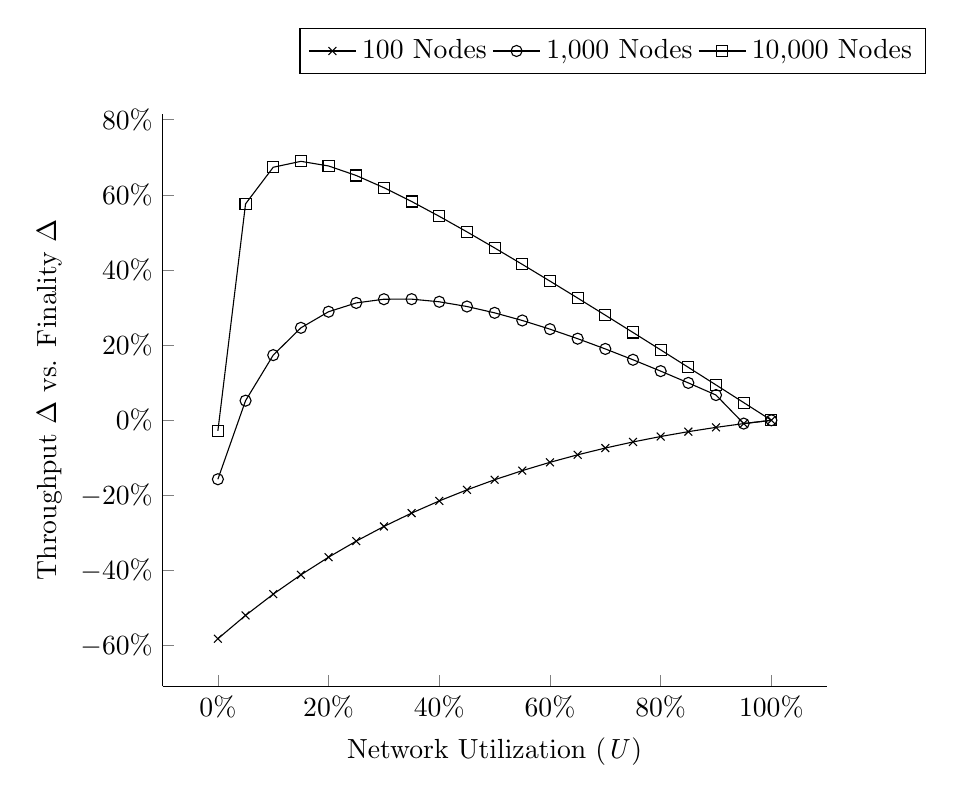
\begin{tikzpicture}
      \pgfplotsset{
          scale only axis,
          xticklabel={\pgfmathparse{\tick*100}\pgfmathprintnumber{\pgfmathresult}\%},
          yticklabel={\pgfmathparse{\tick*100}\pgfmathprintnumber{\pgfmathresult}\%},
          every axis legend/.append style={ at={(1.15,1.15)}, 
          legend columns = 0}
          % legend style={at={(0.5,0.5)},
      }
    
      \begin{axis}[
        % xmode=log,
        % ymode=log,
        axis y line*=left,
        axis x line*=bottom,
        xlabel = Network Utilization (\textit{U}),
        ylabel= Throughput \(\Delta\) vs. Finality \(\Delta\),   
        scaled y ticks=true
      ]

        \addplot[mark=x,color=black] coordinates{
            (1, 0)
            (.95,-0.00875085086638261)
            (.9,-0.0187989993125319)
            (.85,-0.0302313835961472)
            (.8,-0.043142887679075)
            (.75,-0.0576372701980755)
            (.7,-0.0738282268886817)
            (.65,-0.0918406093775239)
            (.6,-0.111811827868503)
            (.55,-0.133893470928493)
            (.5,-0.158253182612207)
            (.45,-0.185076845921641)
            (.4,-0.214571132554597)
            (.35,-0.246966492692794)
            (.3,-0.282520676053356)
            (.25,-0.321522897700105)
            (.2,-0.364298790694081)
            (.15,-0.411216324607017)
            (.1,-0.462692917036203)
            (.05,-0.519204028427371)
            (0,-0.58129361415549)
            % more points
          }; \label{plot_1_y1}
    
        \addplot[mark=o,color=black] coordinates{
            (1, 0)
            (.95,-0.00875085086638261)
            (.9,0.0671847318090388)
            (.85,0.0995370500255989)
            (.8,0.130894988501679)
            (.75,0.161099197548425)
            (.7,0.189954358332614)
            (.65,0.217218427009953)
            (.6,0.242587773750984)
            (.55,0.265676264596652)
            (.5,0.285985195910287)
            (.45,0.302859047758218)
            (.4,0.315418586808512)
            (.35,0.322456529299965)
            (.3,0.322268803136743)
            (.25,0.31236971536466)
            (.2,0.288985767560599)
            (.15,0.246097568383557)
            (.1,0.173476883918847)
            (.05,0.0522287880223851)
            (0,-0.156854896504616)	
            % more points
          }; \label{plot_1_y2}
          
        \addplot[mark=square,color=black] coordinates{
            (1, 0)
            (.95,0.0471276542363689)
            (.9,0.0940968333734938)
            (.85, 0.140880488190999)
            (.8,0.187445042266364)
            (.75,0.233748296740241)
            (.7,0.279736472626588)
            (.65,0.325339945982043)
            (.6,0.370466948376922)
            (.55,0.414994002319199)
            (.5,0.458750930637346)
            (.45,0.501496473543257)
            (.4,0.542876847340344)
            (.35,0.582351483992011)
            (.3,0.61905101794546)
            (.25,0.651482469380805)
            (.2,0.676847892643414)
            (.15,0.689219914258163)
            (.1,0.673468247744901)
            (0.05,0.576068249959748)
            (0,-0.0280081003964768)
            % more points
          }; \label{plot_1_y3}

% 	100 Nodes  (TPS)	1,000 Nodes (TPS)	10,000 Nodes (TPS)
% 100%	0	0	0
% 99%	-0.00165031375594715	0.00684956447079943	0.00943708890651074
% 98%	-0.00334992326651384	0.0136719962067303	0.018868570639354
% 97%	-0.00509945562212089	0.020466591092681	0.0282942767837751
% 96%	-0.00689954859475705	0.0272326204378547	0.0377140321122289
% 95%	-0.00875085086638261	0.0339693298941305	0.0471276542363689
% 94%	-0.0106540222632201	0.0406759383167853	0.0565349532374789
% 93%	-0.0126097339961068	0.0473516365639654	0.0659357312737873
% 92%	-0.0146186689070948	0.053995586231038	0.0753297821629385
% 91%	-0.0166815217224916	0.0606069183156491	0.0847168909377868
% 90%	-0.0187989993125319	0.0671847318090388	0.0940968333734938
% 89%	-0.0209718209578902	0.0737280922088006	0.103469375483743
% 88%	-0.0232007186232419	0.0802360299479392	0.112834272983696
% 87%	-0.0254864372380927	0.0867075387346703	0.1221912707171
% 86%	-0.027829734985105	0.0931415737969925	0.131540102044715
% 85%	-0.0302313835961472	0.0995370500255989	0.140880488190999
% 84%	-0.0326921686563201	0.105892840008188	0.150212137545661
% 83%	-0.0352128899162063	0.112207771947697	0.159534744916431
% 82%	-0.0377943616125981	0.118480627456378	0.168847990729
% 81%	-0.0404374127979855	0.124710139216991	0.178151540169741
% 80%	-0.043142887679075	0.130894988501679	0.187445042266364
% 79%	-0.0459116459646319	0.137033802538329	0.196728128901203
% 78%	-0.0487445632229522	0.143125151713345	0.206000413751314
% 77%	-0.0516425312492659	0.149167546598887	0.215261491148955
% 76%	-0.0546064584434062	0.155159434791552	0.224510934855392
% 75%	-0.0576372701980755	0.161099197548425	0.233748296740241
% 74%	-0.0607359092980535	0.16698514620517	0.242973105357741
% 73%	-0.0639033363307175	0.172815518359506	0.252184864410451
% 72%	-0.0671405301082428	0.178588473801943	0.261383051089853
% 71%	-0.0704484881018747	0.184302090174034	0.270567114282188
% 70%	-0.0738282268886817	0.189954358332614	0.279736472626588
% 69%	-0.0772807826112031	0.195543177396536	0.288890512411124
% 68%	-0.0808072114504299	0.201066349450237	0.298028585290751
% 67%	-0.0844085901125768	0.206521573876075	0.30715000580932
% 66%	-0.08808601633011	0.211906441284722	0.316254048705741
% 65%	-0.0918406093775239	0.217218427009953	0.325339945982043
% 64%	-0.0956735106023761	0.22245488413093	0.334406883708403
% 63%	-0.0995858839721068	0.227613035981431	0.343453998537203
% 62%	-0.103578916637198	0.232689968101487	0.352480373894715
% 61%	-0.107653819511241	0.23768261958238	0.361485035815107
% 60%	-0.111811827868503	0.242587773750984	0.370466948376922
% 59%	-0.116054201959627	0.247402048133861	0.379425008697098
% 58%	-0.120382227646092	0.252121883635285	0.388358041431626
% 57%	-0.124797217054114	0.256743532856419	0.397264792725189
% 56%	-0.129300509248689	0.261263047475068	0.406143923544275
% 55%	-0.133893470928493	0.265676264596652	0.414994002319199
% 54%	-0.138577497142414	0.26997879197721	0.423813496809984
% 53%	-0.143354012028482	0.274165992008181	0.432600765098886
% 52%	-0.148224469576048	0.278232964340179	0.44135404559816
% 51%	-0.153190354412039	0.282174527008895	0.450071445945142
% 50%	-0.158253182612207	0.285985195910287	0.458750930637346
% 49%	-0.163414502538282	0.289659162454145	0.467390307237591
% 48%	-0.168675895702019	0.293190269204561	0.475987210952416
% 47%	-0.174038977657137	0.296571983292516	0.484539087355514
% 46%	-0.179505398920214	0.29979736735919	0.493043172990538
% 45%	-0.185076845921641	0.302859047758218	0.501496473543257
% 44%	-0.190755041987778	0.305749179710422	0.509895739220138
% 43%	-0.196541748355527	0.308459409064707	0.518237436907147
% 42%	-0.202438765220558	0.310980830273137	0.526517718606584
% 41%	-0.208447932820523	0.313303940135568	0.534732385558236
% 40%	-0.214571132554597	0.315418586808512	0.542876847340344
% 39%	-0.220810288140806	0.317313913502764	0.550946075111317
% 38%	-0.227167366812617	0.318978296212942	0.558934547988946
% 37%	-0.233644380556359	0.320399274727637	0.566836191362599
% 36%	-0.240243387391116	0.321563476058732	0.574644305686068
% 35%	-0.246966492692794	0.322456529299965	0.582351483992011
% 34%	-0.253815850564154	0.323062970774183	0.589949515987391
% 33%	-0.260793665252686	0.323366138151968	0.597429276112036
% 32%	-0.267902192618279	0.323348052016039	0.604780592342059
% 31%	-0.275143741652748	0.322989283099795	0.611992091759971
% 30%	-0.282520676053356	0.322268803136743	0.61905101794546
% 29%	-0.290035415852594	0.321163816910848	0.625943013999696
% 28%	-0.297690439106577	0.319649572684094	0.632651863413209
% 27%	-0.305488283644525	0.317699147682258	0.639159178901855
% 26%	-0.313431548881925	0.315283204724551	0.645444026599893
% 25%	-0.321522897700105	0.31236971536466	0.651482469380805
% 24%	-0.329765058395059	0.308923644040806	0.657247008246536
% 23%	-0.338160826698525	0.304906586674421	0.662705894216418
% 22%	-0.346713067874472	0.300276355864411	0.667822274283021
% 21%	-0.355424718894278	0.294986503237705	0.672553122797663
% 20%	-0.364298790694081	0.288985767560599	0.676847892643414
% 19%	-0.373338370517947	0.282217434791059	0.680646796554293
% 18%	-0.382546624350676	0.274618593231741	0.683878594596515
% 17%	-0.391926799444289	0.266119263159504	0.686457713938461
% 16%	-0.40148222694241	0.2566413755391	0.688280453366783
% 15%	-0.411216324607017	0.246097568383557	0.689219914258163
% 14%	-0.421132599652237	0.234389761609904	0.689119129925581
% 13%	-0.431234651690136	0.221407461328243	0.687781599247454
% 12%	-0.441526175793677	0.20702573167703	0.684958003600565
% 11%	-0.452010965682347	0.191102755593143	0.680327182460175
% 10%	-0.462692917036203	0.173476883918847	0.673468247744901
% 9%	-0.473576030944429	0.153963043092706	0.663818616294178
% 8%	-0.48466441749481	0.132348332653256	0.650608901715372
% 7%	-0.495962299510891	0.108386591050549	0.632758272932124
% 6%	-0.507474016443957	0.081791636236959	0.60869912111628
% 5%	-0.519204028427371	0.0522287880223851	0.576068249959748
% 4%	-0.531156920501221	0.0193041400804878	0.531128814459303
% 3%	-0.543337407015695	-0.0174491475540527	0.467602553340845
% 2%	-0.555750336222049	-0.0585885477774608	0.374066687520415
% 1%	-0.568400695060574	-0.104785282879006	0.227326975834317
% 0%	-0.58129361415549	-0.156854896504616	-0.0280081003964768
        
        \addlegendimage{/pgfplots/refstyle=plot_1_y1}\addlegendentry{100 Nodes}
        \addlegendimage{/pgfplots/refstyle=plot_1_y2}\addlegendentry{1,000 Nodes}
        \addlegendimage{/pgfplots/refstyle=plot_1_y3}\addlegendentry{10,000 Nodes}

        \end{axis}
    \end{tikzpicture}
    \caption{The percentage change in throughput versus the change in finality as \textit{network utilization} is reduced.}
    \label{fig:comp_change}
\end{figure}
Observing the graphs for network sizes of 100, 1,000, and 10,000 nodes over variable utilization rates (see \textit{Figure} \ref{fig:comp_change}), it is clear that as the network size increases the moment of ideal utilization, represented by the maximum value of each distribution, moves to lower rates of utilization. This can be further proven when calculating the exact moment of \textit{ideal utilization} using the differential equation, the results of which are displayed in \textit{Table} \ref{tab:tab1}.
\begin{table}[!h]
\centering
    \begin{tabular}{cccc}
     \hline
     \textbf{$n$}& Ideal $U$ $\%$ & Fin $\%$ Reduc.&TPS $\%$ Reduc.\\
     \hline
     100   & 100 $\%$   &0.0 $\%$&   0.0 $\%$\\
     1000&   32.55 $\%$ & 56.82 $\%$  &24.61 $\%$\\
     10000& 14.58 $\%$ & 95.02 $\%$&  34.65 $\%$\\
     \hline
    \end{tabular}
    \caption{The \textit{ideal utilization} of the distributions graphed in \textit{Figure} \ref{fig:comp_change} with the relative reductions in finality and throughput.}
    \label{tab:tab1}
\end{table}
